\documentclass[11pt]{article}
\usepackage[margin = 1in]{geometry}
\usepackage{amsmath}
\usepackage{amssymb}
\usepackage{amsthm}
\usepackage{graphicx}
\usepackage{subfig}
\usepackage{enumitem}
\usepackage{url}
\usepackage[parfill]{parskip}
\newcommand{\skipline}{\vspace{\baselineskip}}
\newenvironment{problem}[1]{\textbf{Problem #1: }}{\newpage}


\begin{document}
	
	\begin{center}
		\textbf{Assignment 1} \\
		\textbf{Computer Vision} \\
		\textbf{CS 559} \\
		\textbf{Stephen Giang, RedID: 823184070} \\
	\end{center}

	\begin{problem}{1}
		\begin{enumerate}[label = (\alph*)]
			\item What is an interchange format? 
			\\ \\
			Interchange format is a format of an image designed to facilitate the exchange of image data between users
			\item Give three examples of interchange formats.
				\begin{enumerate}[label = (\roman*)]
					\item GIF (Graphic Interchange Format) 
					\item PNG (Portable Network Graphics)
					\item PGM (Portable Gray Format)
				\end{enumerate}
			\item What is the signature of a PGM format. Give two examples of the signature.
			\\ \\
			The signature of a PGM format are signatures with different image types and storage types. One example would be the signature P1, which has an image type of binary and a storage type of ASCII.  Another example would be signature P5, which has an image type of greyscale and a storage type of raw byte.
			\item What is patterning in printing? 
			\\ \\
			Patterning in printing is a method where each pixel is replaced by a pattern taken from a binary font.
			\item Explain the principle and operation of error diffusion for printing.
			\\ \\
			The way error diffusion works is that we take the original image and turn it into another image.  In a black-white example, if the pixel $f(x,y)$ is more dark, then it will turn into a black pixel.  If the pixel is more white , then it will turn into a white pixel.  However, for pixels that are in the middle and not too dark or too light, we use Dithering by error diffusion.  This will convert the pixel, and turn it into a black or white pixel depending on if $f(x,y) > 128$ or not.  Then because the difference between the original color and the new color (black or white) will be so high, we take the difference and multiply it by a certain Error diffusion factor and add it to the surrounding pixels making the surrounding pixels a similar color to the new color.  This way, the human eye will then average the brightnesses to make a coherent image.
		\end{enumerate}
	\end{problem}

	\begin{problem}{2}
		In an automated manufacturing, inspection of circuit boards is to be done using a CCD camera. The individual imaging elements (photosites) each has a dimension of 5 by 5 $\mu$m (micron) and the spacing between the elements is 1 $\mu$m. The circuit boards are 60 by 60 mm, and defects appear as dark circular blobs with diameter of 0.4 mm or larger.  The smallest defect must appear in the image as an area of at least 6 by 6 pixels. Assume that available lenses come with focal lengths of multiple of 25 mm, 35 mm and 50 mm, and the available camera resolutions are multiple of 256 by 256 pixels up to 2048 by 2048 pixels (4 Mpix).  Manufacturing requirements dictate that distance between camera and the circuit board must be between 200 mm to 500 mm. The image of the board must occupy the whole image plane. You are to select the lens focal length and the minimum camera resolution (number of pixels) required.  Show in reasonable details the analysis that lead to your answers. This assignment does not need any programming. 
		\\ \\
		Notice that the defect is a circle with a $0.4$mm diameter.  Also notice that the defect must fit in an area of at least 6 by 6 pixels.  If we circumscribe the circle inside the 6 by 6 square, we get that $.4$mm $= 6$ pixels.  Because one side of the entire circuit board is 60mm, we can do a simple proportion, and get that the 60 by 60 mm circuit board has a 900 by 900 pixel resolution.  Because resolutions come in multiples of 256 pixels, we need at least a resolution of 1024 by 1024 pixels.  Now we can multiply the resolution by the size of the photosite plus spacing.  So that we get the image size, $x = (5 + 1)(1024)\mu m = 6144\mu m = 6.144mm$.  We have the object size, $X = 60mm$. 
		\begin{align*}
			\frac{x}{f} &= \frac{X}{Z - f} \\
			\frac{6.144}{f} &= \frac{60}{Z - f} \\
			6.144Z - 6.144f &= 60f \\
			Z &= 10.765625f
		\end{align*}  
		Now if we apply that $Z \in {[200,500]}$, we get the following:
		\begin{center}
			$200 \leq 10.765625f \leq 500$ \\
			$18.577 \leq f \leq 46.444$
		\end{center}
		Now we get the range of values of $f \in {[18.577, 46.444]}$.  Because $f$ is a multiple of 25 mm, 35 mm, and 50 mm, we get that for our problem that $f = 25$ or $f = 35$
	\end{problem}

	\begin{problem}{3}
		What is the storage saving in terms of $b$ and $c$ when reducing a b bit image into $c < b$ bit image? Write a program to reduce an $b=8$ bit image into a $c<8$ bit image. Do not use the Matlab or Python library, but you can look their function/method to get ideas. Apply your code to the following 8-bit image, with $c=4$.  Show the output image. 
		\\ \\
		We have that storage for a $b$-bit image is $\frac{wh * (b)}{8}$ bytes. The storage saving in terms of $b$ and $c$ would be $1 - \frac{c}{b}$ the original storage.  So converting from an 8-bit to 4-bit image will save half the original storage. Converting a 16-bit to a 1-bit, you would end up with $\frac{1}{16}^{th}$ the original storage but saving $\frac{15}{16}^{th}$ the original storage. Converting a $b$-bit image into a $c$-bit image is going to be a factor of two for each bit reduced. (Code down Below)
		\begin{figure}[h!]
			\text{8 - Bit (Original)} \\
			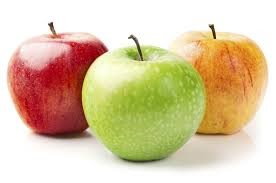
\includegraphics[width = 15cm, height = 8cm]{../Photos/Apples8Bit.jpg}
			\\
			\text{4 - Bit (Notice the "shine" on the green apple to see the difference between 8 and 4 bit)} \\
			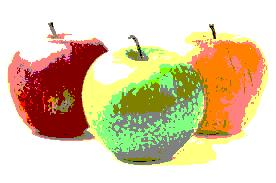
\includegraphics[width = 15cm, height = 8cm]{../Photos/Apples4Bit.jpg}
		\end{figure}
	\end{problem}
	
	\begin{problem}{4}
		The purpose of this program is to understand the representation and manipulation of colors in an image. Consider a color image and suppose we want to keep a particular object in the image in its original color and turn other parts of the image into greyscale. As an example is the image (a) below that should turn into image (b). Write a program to achieve this, and apply your program to two images of your choice to demonstrate the effectiveness of your program.
		\begin{figure}[h!]
			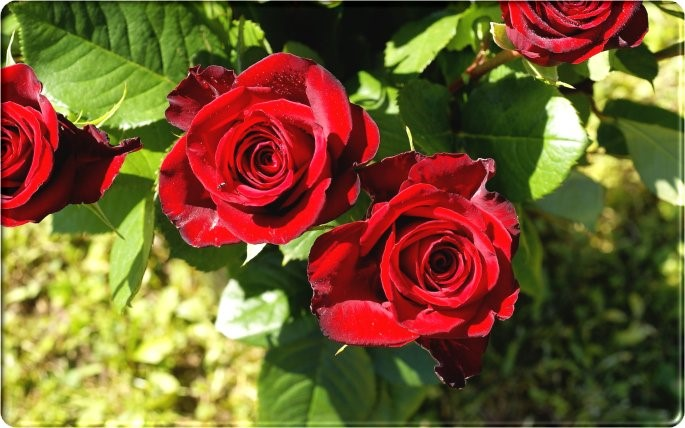
\includegraphics[width = 8cm, height = 5cm]{../Photos/FlowersFullColor.jpg}
			\hspace{.75cm}
			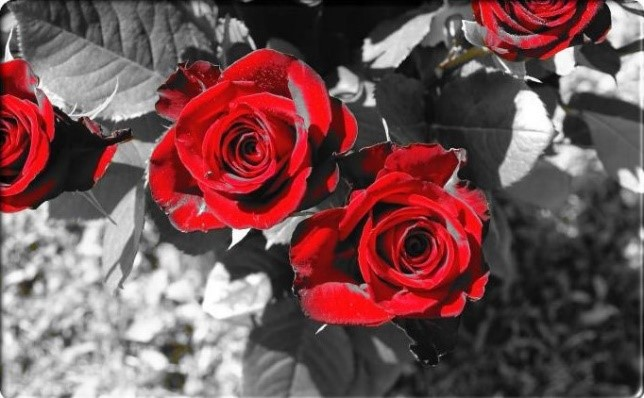
\includegraphics[width = 8cm, height = 5cm]{../Photos/FlowersRedRoses.jpg}
		\end{figure}
		\\
		\text{}\hspace{4cm}(a)\hspace{8.75cm}(b)
		\\ \\
		\begin{enumerate}
			\item Flowers Example:
			\begin{figure}[h!]
				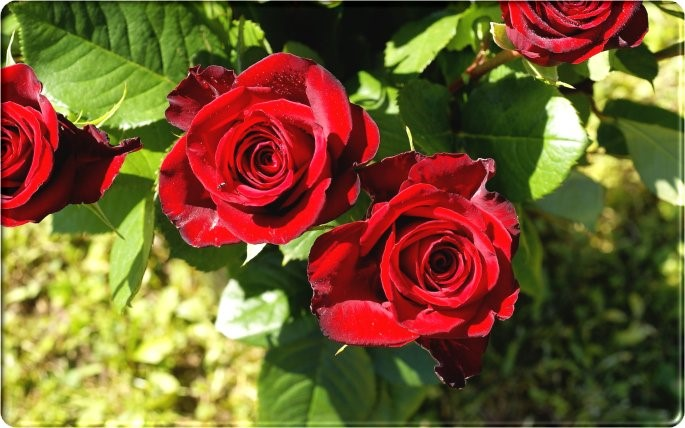
\includegraphics[width = 8cm, height = 5cm]{../Photos/FlowersFullColor.jpg}
				\hspace{.75cm}
				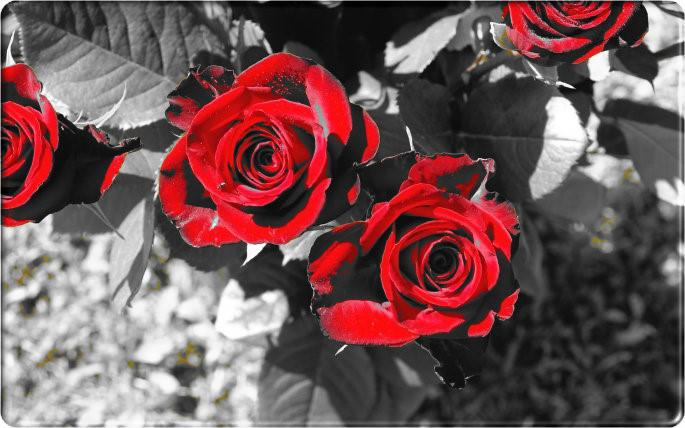
\includegraphics[width = 8cm, height = 5cm]{../Photos/FlowersResults.jpg}
			\end{figure}
		\\ \\
		My reasoning behind programming this started with reading the original image.  I first extracted the RGB matrices and then took the original image and made a black and white version.  Now I had to find a way to find the pixels with the specified color. I used a nested for loop that loops through all of the pixels, and checked if the original pixel consisted of more of the specified color than the other colors.  For the Flowers Example, I checked each pixel to see if red was more than 128 and if green and blue were less than 128. If so, I looped through the z component of the pixel (the component that determines whether red,green,blue), and reinserted the original color back in the pixel.  I do this for all pixels, and it simply finds the pixels with the specified color, and reinserts the original color back.  I had to make sure the finding parameter (more one color, less other colors) was the way I did so, to truly isolate the pixels that we majority of the specified color.  
			\newpage
			\item Example 1:
			\begin{figure}[h!]
				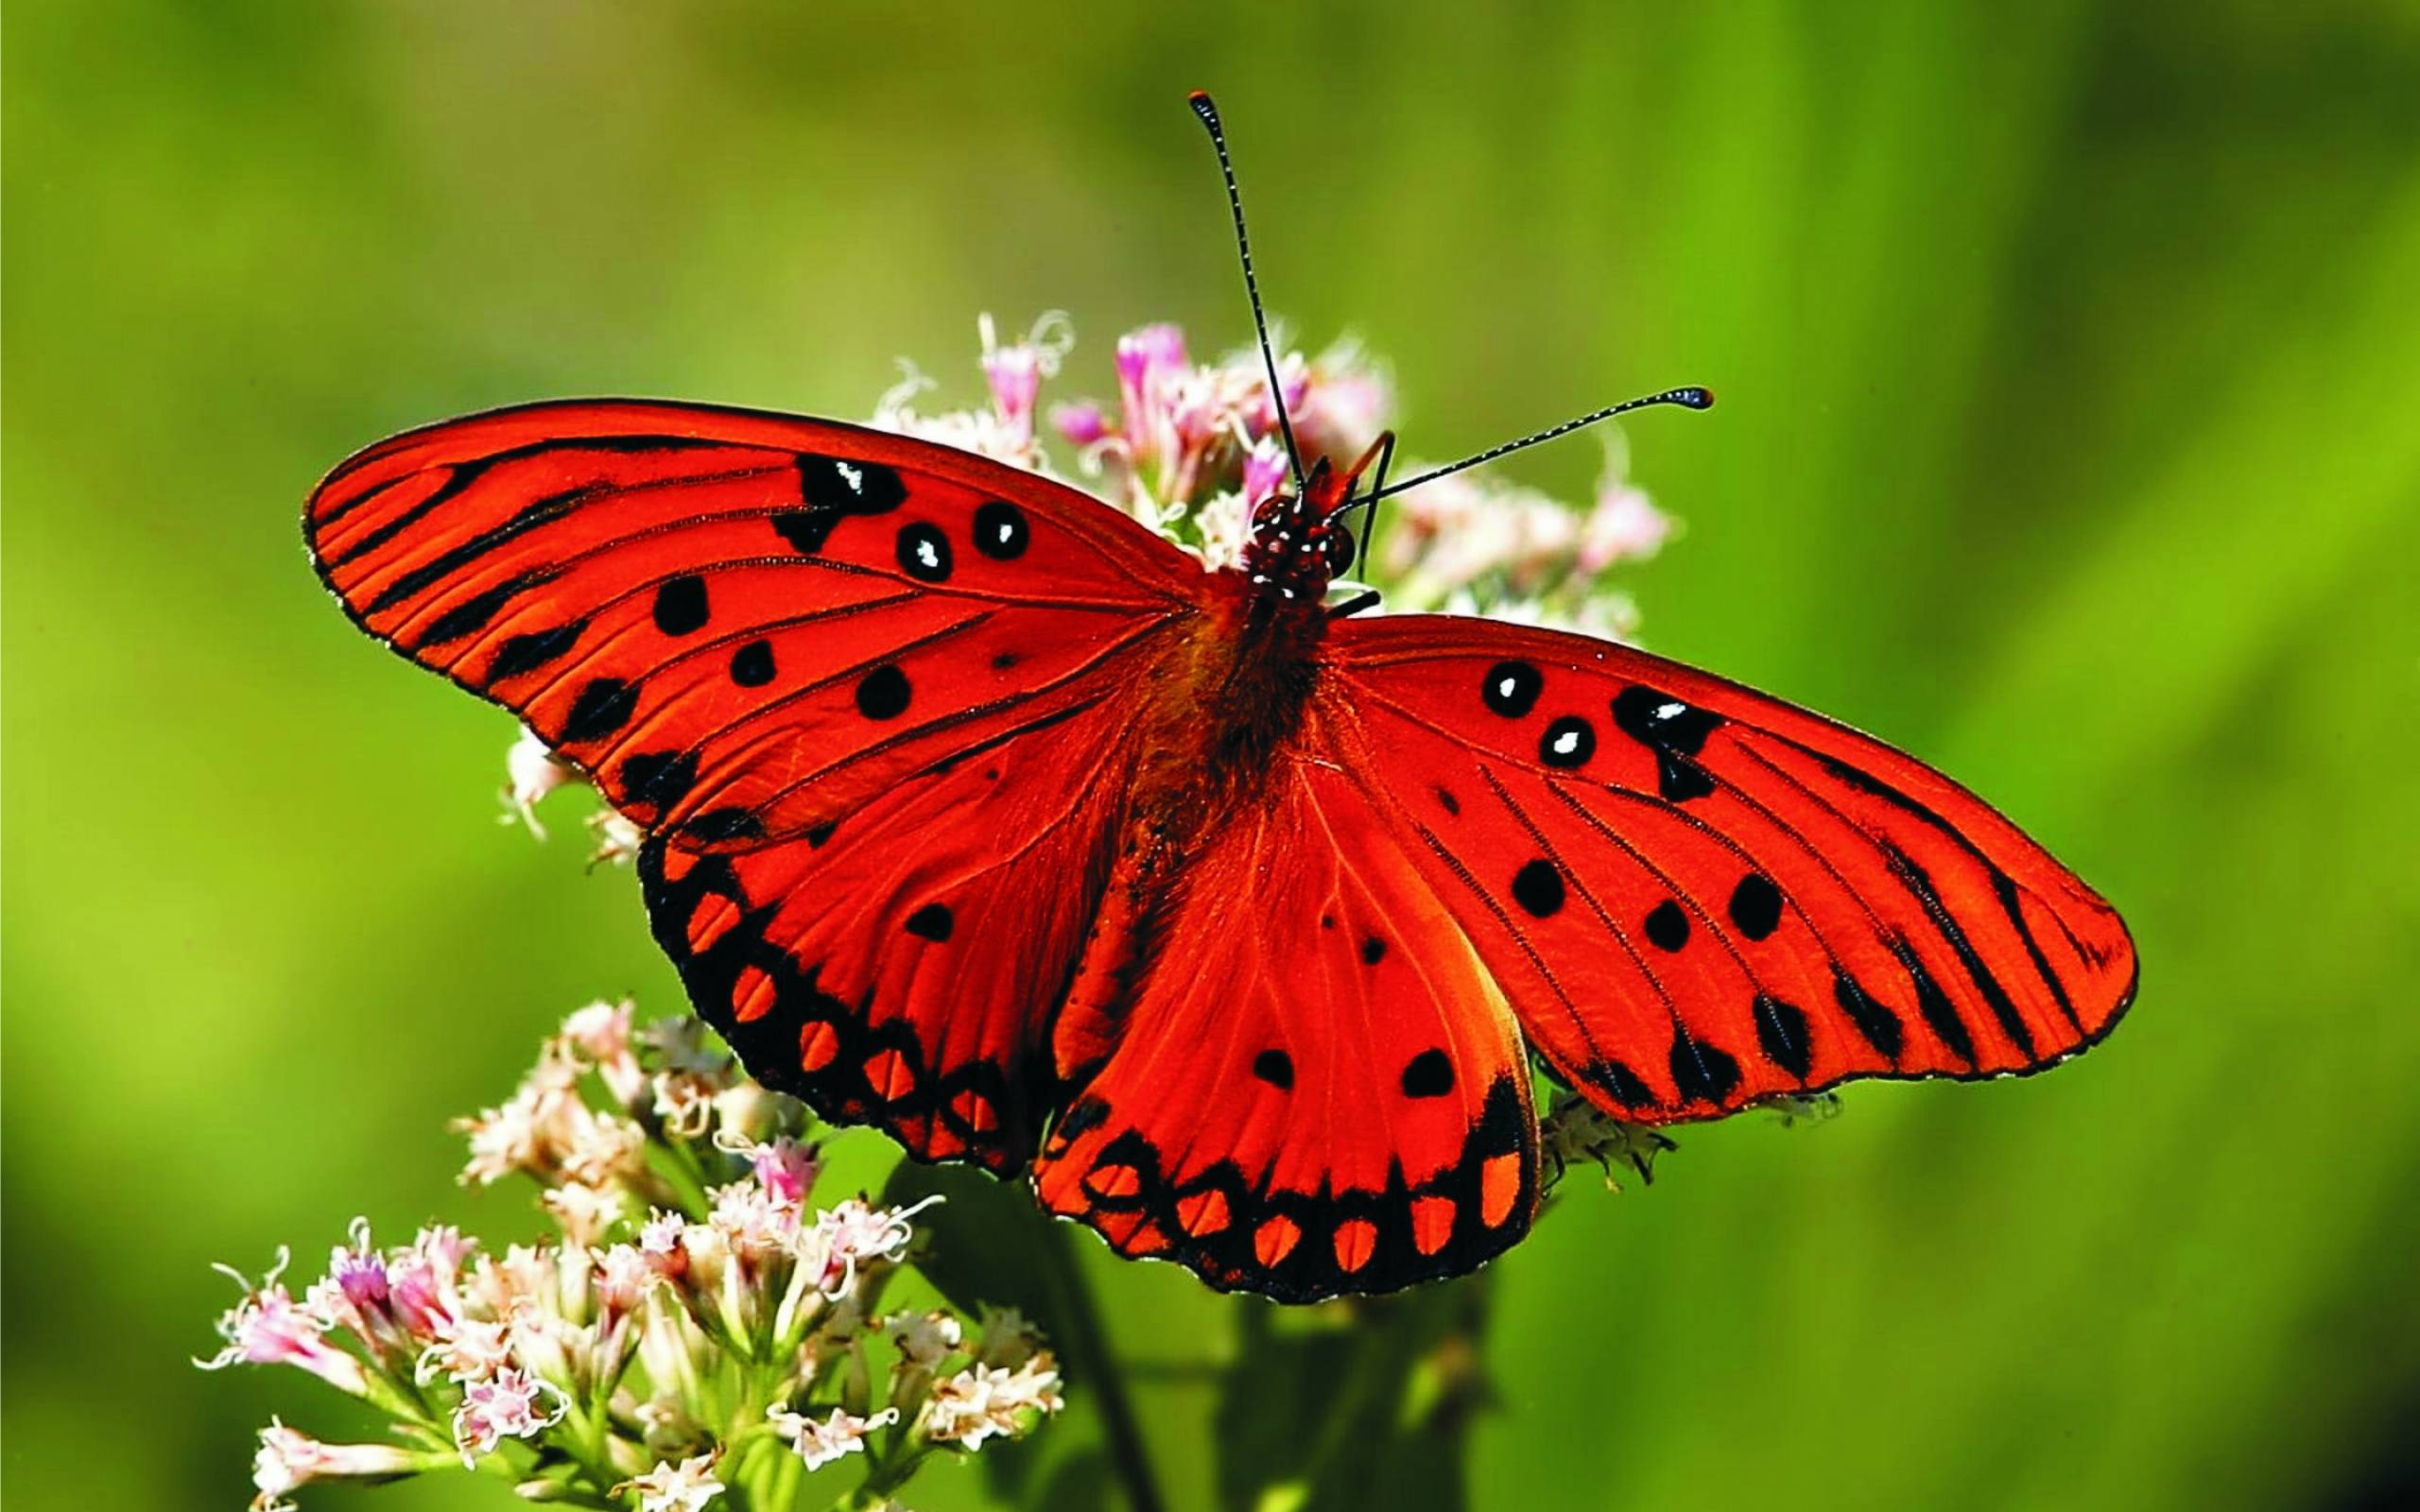
\includegraphics[width = 8cm, height = 5cm]{../Photos/Test1.jpg}
				\hspace{.75cm}
				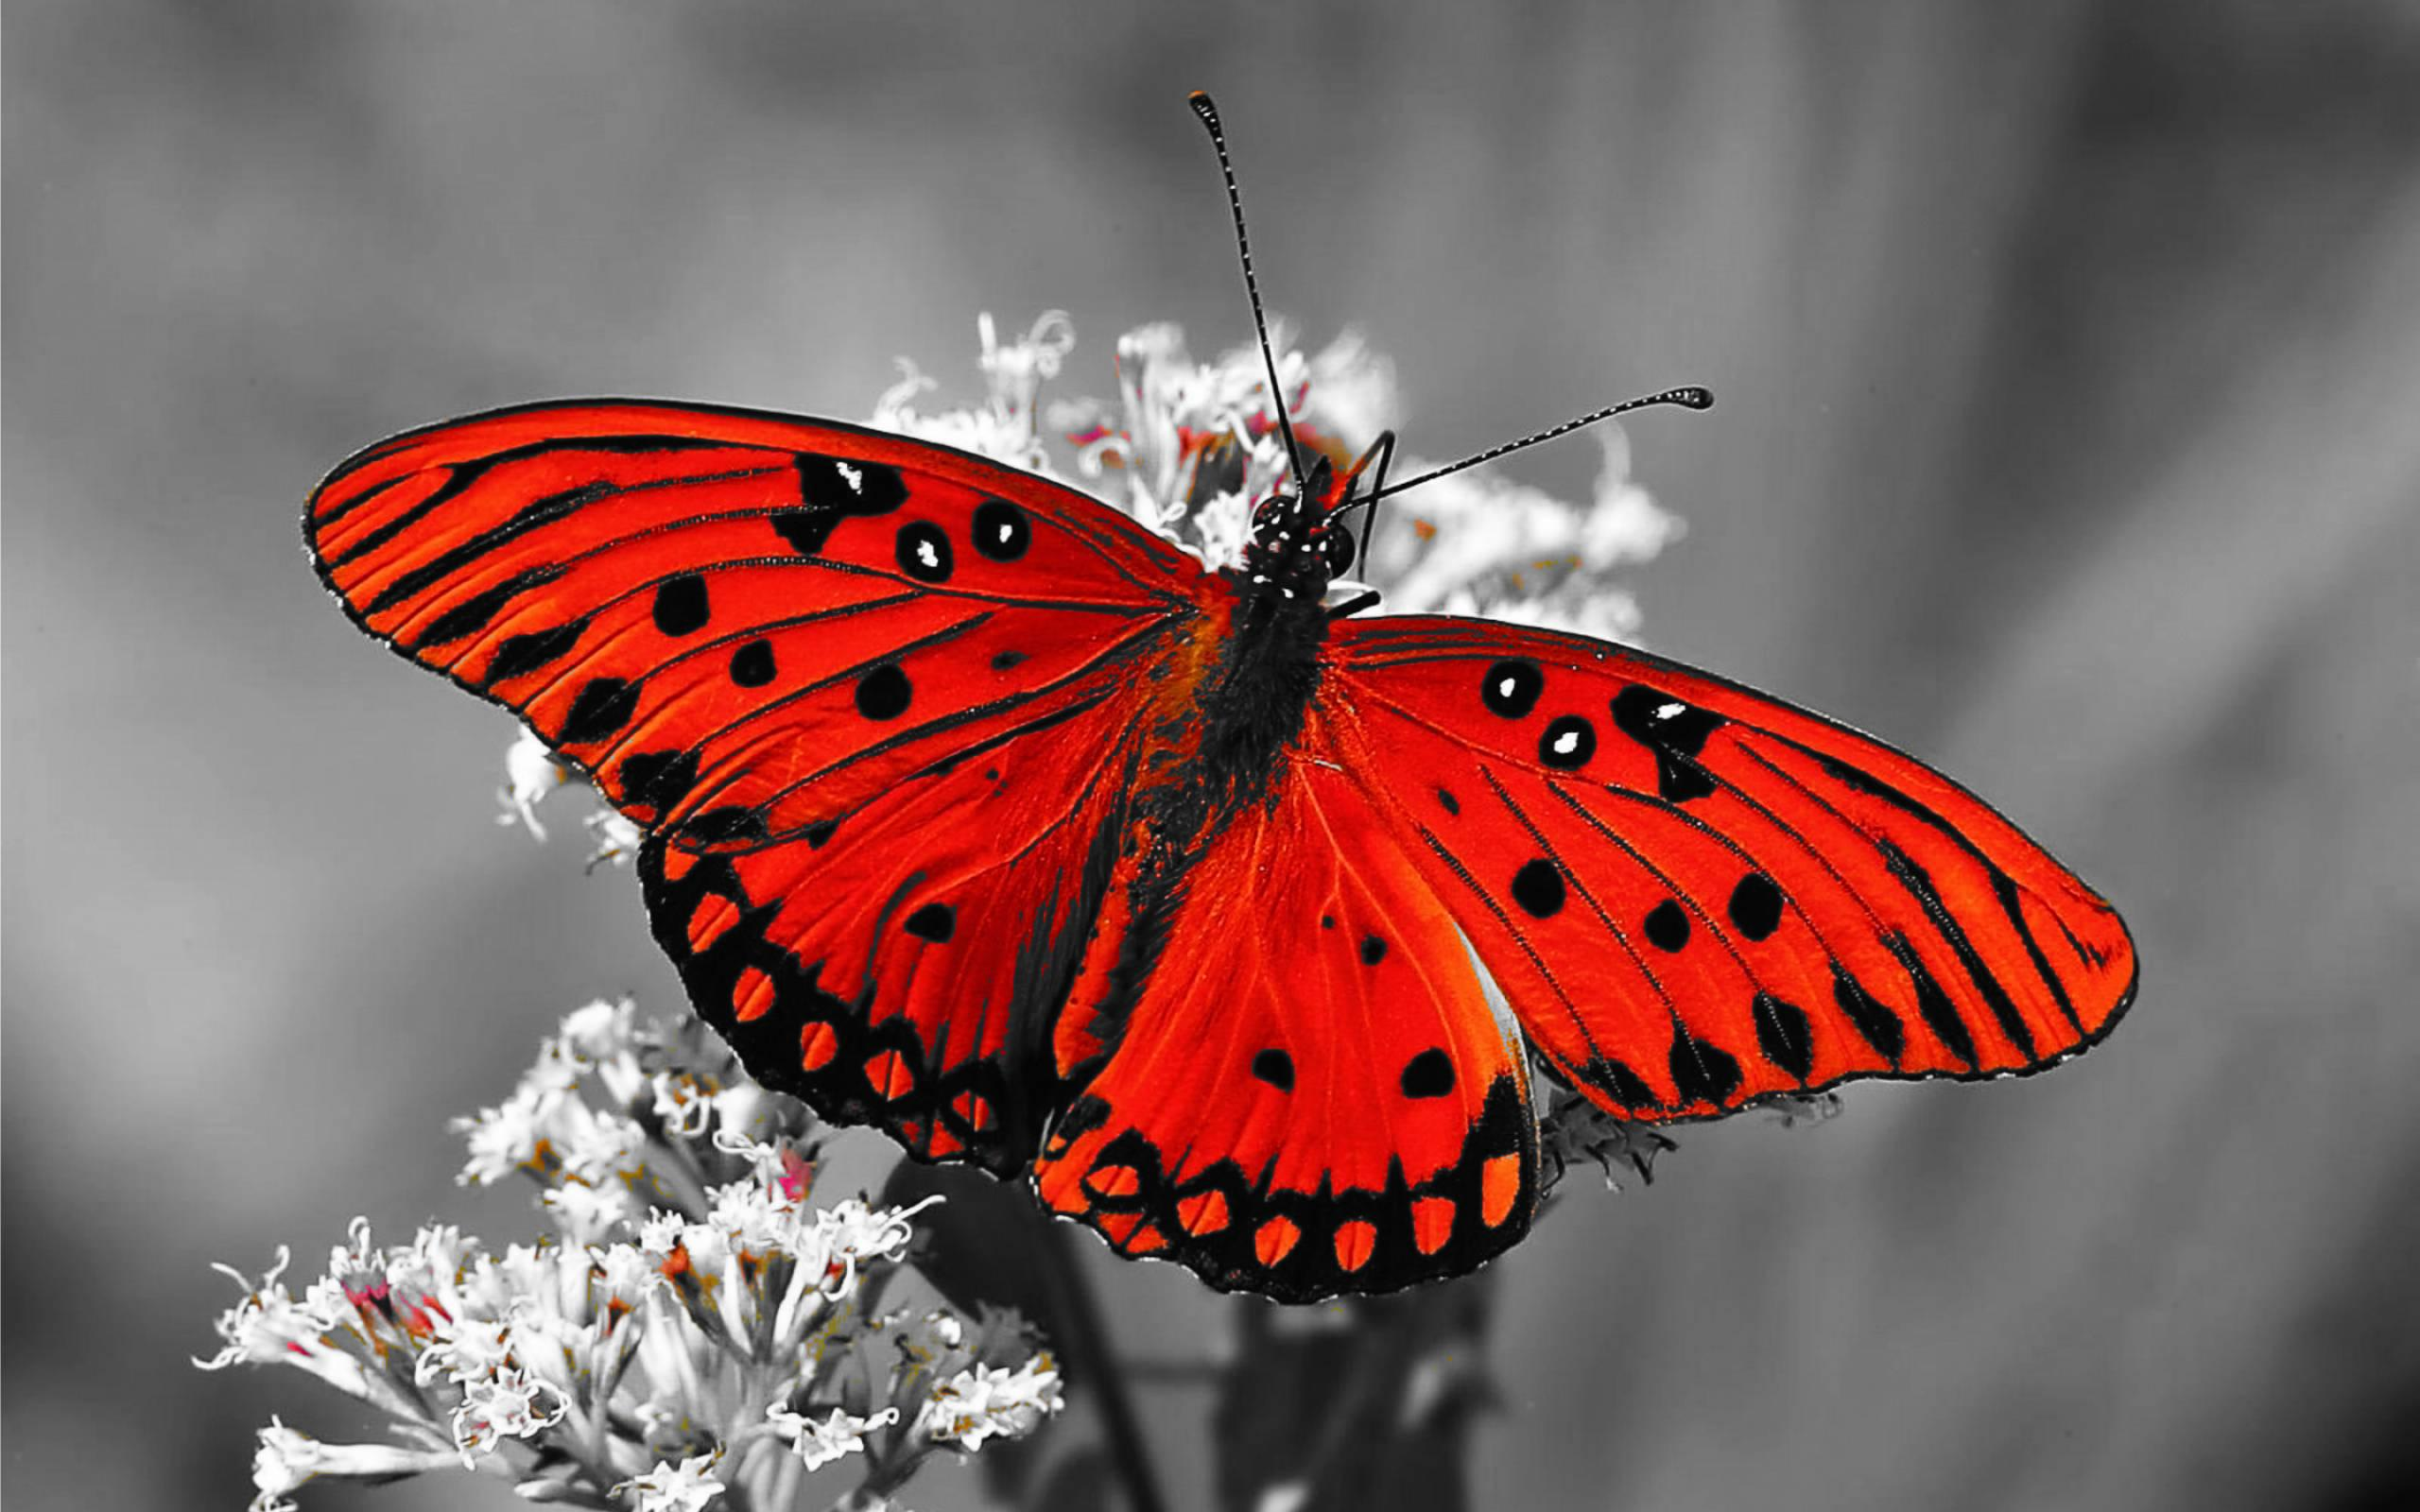
\includegraphics[width = 8cm, height = 5cm]{../Photos/Test1Results.jpg}
			\end{figure}
			\item Example 2:
			\begin{figure}[h!]
				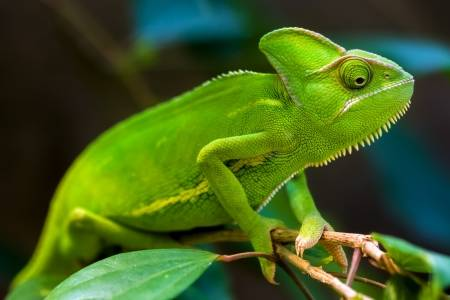
\includegraphics[width = 8cm, height = 5cm]{../Photos/Test2.jpg}
				\hspace{.75cm}
				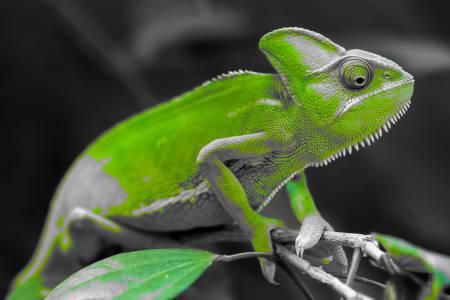
\includegraphics[width = 8cm, height = 5cm]{../Photos/Test2Results.jpg}
			\end{figure}
			\item Example 3:
			\begin{figure}[h!]
				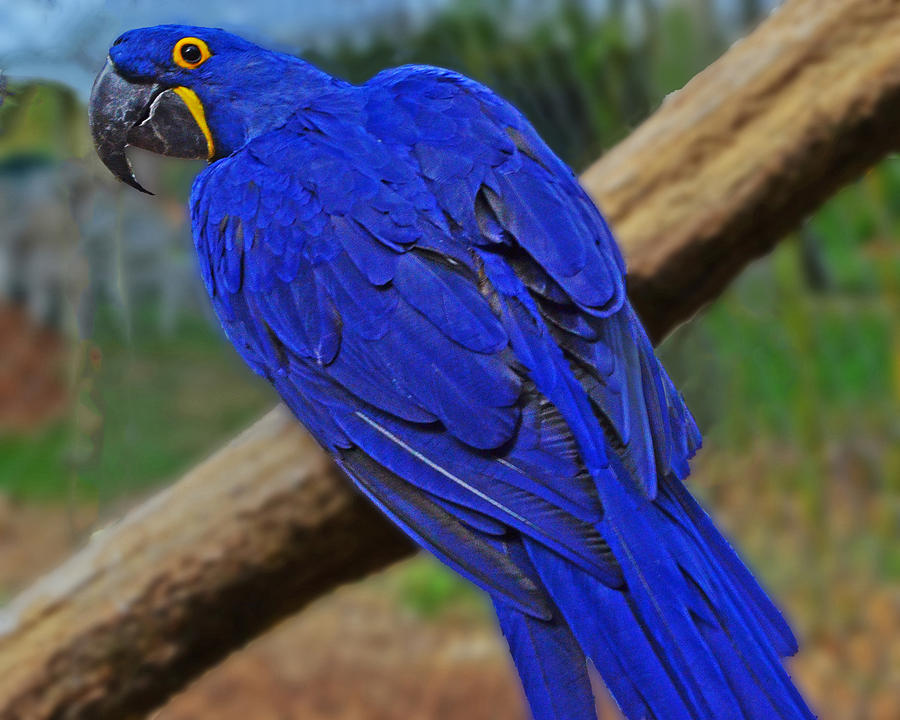
\includegraphics[width = 8cm, height = 5cm]{../Photos/Test3.jpg}
				\hspace{.75cm}
				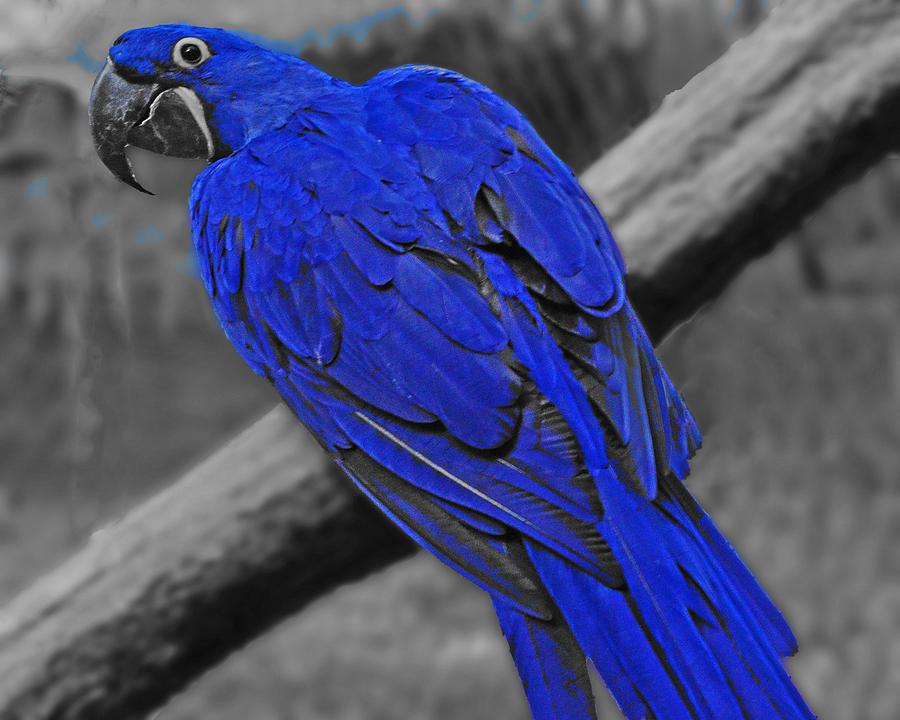
\includegraphics[width = 8cm, height = 5cm]{../Photos/Test3Results.jpg}
			\end{figure}
		\end{enumerate}
		
	\end{problem}


\end{document}
